%---------------------------------------------------------------------------%
%-                                                                         -%
%-                           LaTeX Template                                -%
%-                                                                         -%
%---------------------------------------------------------------------------%
%---------------------------------------------------------------------------%
%->> Document class declaration
%---------------------------------------------------------------------------%
\documentclass{Style/soundresearch}%
%- Multiple optional arguments:
%- [<oneside|twoside|print>]% oneside eprint, twoside eprint, or paper print
%- [fontset=<adobe|...>]% specify font set to replace automatic detection
%- [plain]% thesis writing of international students
%- [draftversion]% show draft version information
%- [standard options for ctex article class: draft|paper size|font size|...]%
%---------------------------------------------------------------------------%
%->> Document settings
%---------------------------------------------------------------------------%
\usepackage[numbers,xhf]{Style/artratex}% document settings
%- usage: \usepackage[option1,option2,...,optionN]{artratex}
%- Multiple optional arguments:
%- [bibtex|biber]% set bibliography processor and package
%- [<numbers|super|authoryear|alpha>]% set citation and reference style
%- <numbers>: textual: Jones [1]; parenthetical: [1]
%- <super>: textual: Jones superscript [1]; parenthetical: superscript [1]
%- <authoryear>: textual: Jones (1995); parenthetical: (Jones, 1995)
%- <alpha>: textual: not available; parenthetical: [Jon95]
%- [geometry]% reconfigure page layout via geometry package
%- [lscape]% provide landscape layout environment
%- [xhf]% disable header and footer via fancyhdr package
%- [color]% provide color support via xcolor package
%- [background]% enable page background
%- [tikz]% provide complex diagrams via tikz package
%- [table]% provide complex tables via ctable package
%- [list]% provide enhanced list environments for algorithm and coding
%- [math]% enable some extra math packages
%- [xlink]% disable link colors
\usepackage{Style/artracom}% user defined commands

\setcounter{tocdepth}{1}
%\usepackage[UTF8]{ctex}
%---------------------------------------------------------------------------%
%->> Document inclusion
%---------------------------------------------------------------------------%
%\includeonly{Tex/Chap_1,...,Tex/Chap_N}% selected files compilation
%---------------------------------------------------------------------------%
%->> Document content
%---------------------------------------------------------------------------%
%-
%-> Titlepage information
%-
%---------------------------------------------------------------------------%
%->> Titlepage information
%---------------------------------------------------------------------------%
%-
%-> 中文封面信息
%-

%---------------------------------------------------------------------------%
%---总体信息
\projectname{煤炭行业生产端废水无害化处理方式研究}
\id{RD03}
\project{煤炭行业生产端废水无害化处理技术}
\projectlocation{安徽铜陵城北污水处理厂}
\manager{解建坤}
\department{设计研究院}
\company{北京桑德环境工程有限公司}
\managergender{男}
\managerbirth{1982.03}
\managerethnic{汉}
\managerdegree{博士}
\managertitle{高级工程师}
\managerarea{水处理工艺研发}
\managertelephone{15810355385}
\manageremail{xiejiankun@soundglobal.cn}

%---开题信息
\attendant{许慧英、仝延忠、白利云、彭永立、张锦祥}
\expectperiod{2018年1月-2018年12月}
\fund{900万元}
\fundtype{公司自筹}
\achievementmiddle{中期:初步取得处理煤炭行业生产端废水的Fenton试剂投加量}
\achievementfinal{末期:在生产中验证工艺处理煤炭行业生产端废水的稳定性}
\projectarea{水处理工艺开发}
\projectdirection{工业废水等难降解污水深度处理}
\projectabstract{\setlength{\parindent}{2em}\qquad煤炭行业生产端废水多种多样,有煤矿开采中产生的煤层气废水,如压裂液和采气排水,也有煤炭制焦过程产生的焦化废水,这系列的废水具有高矿化度,高盐度,难以生物处理等特点,若不经处理直接排放,必然对环境产生恶劣影响。本次主要针对煤炭行业生产端废水进行工艺开发,确定处理该类废水的主要工艺方案,并通过设计、制造、安装、调试运行等工作,在煤炭行业生产端废水处理领域建立一套完整的水处理体系,保证运行出水结果稳定达标,为公司在煤化工行业打开新的市场。
}

%---结题信息
\attendantchanged{许慧英、仝延忠、白利云、彭永立、张锦祥(无变化)}
\actualperiod{2018年1月-2018年12月}
\actualfund{860.97万元}
\actualfundtype{公司自筹}
\actualachievementmiddle{中期:初步取得药剂投加量,并对实验进行优化.}
\actualachievementfinal{末期:结合生产,验证Fenton工艺处理焦化废水的稳定性}
\jietiabstract{\par强化芬顿技术为核心的高级催化氧化工艺适用于煤化工废水处理领域,可解决\showproject中存在的难题。课题中发现焦化废水水质水量波动大,以水质形状作为投药和调节pH的指标既满足处理效果又降低运行成本。此外,水质中TDS极高并含有高浓度的硫化物易产生浮泥和发臭问题,需降低沉淀池表面负荷,延长沉淀池的停留时间,同时投加硫酸亚铁,可去除水中的硫化物及少部分的还原性物质。\par
}
%
%\title{title}{subtitle}
\title{研究开发项目中期进展报告}{}
\applydate{2017年12月}
\begin{document}
%-
%-> Frontmatter: title page, abstract, content list, symbol list, preface
%-
\pagenumbering{roman}% page numbers with roman style
\maketitle% title page, abstract
%-
%-> Mainmatter
%-
\clearpage
\pagenumbering{arabic}% restart page numbers with arabic style

\makezhongqiinfo
\vspace{-4.4mm}\begin{longtable}{|p{156mm}|}
    \hline
    \endfirsthead
    \hline
    \endhead
    \hline
    \endfoot
    \hline
    \setlength{\parindent}{2em}
    {\bfseries研发项目进度情况:}(立项实施以来的研发工作概况;资料调研和社会调查情况;已完成的研究工作;对照原定的研究计划,如果未能按计划进行,请说明具体原因。)\par
    按照研究计划,本阶段开展了如下工作:\par
1、参考了大量中英文文献,对当前\showproject有了较为全面的了解;\par
2、完成了试验装置的设计及设备材料采购工作,并加工制作完试验装置;\par
3、以\showprojectlocation焦化废水为研究对象完成试验,开展处理工艺效果及影响因素研究,对运行参数进行调整和优化。\par \\[200mm]
    \hline 
    \setlength{\parindent}{2em}
    {\bfseries已取得的阶段性成果:} \par
    经过生物滴滤池15d的稳定运行后,在温度为25-30℃,循环液pH值控制在6.5-7.0,气流量为9000m3/h的条件下,生物滤池对的氨及硫化氢的降解效果如下图。\par
{\noindent  \centering  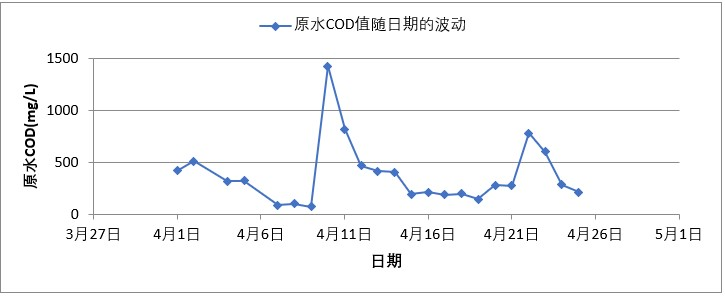
\includegraphics[width=150mm]{Img/fig1.jpg}\par}
{\hspace{40mm} 
图1 氨的进、出气浓度及去除率}
\vspace{10mm}
\par
{\noindent    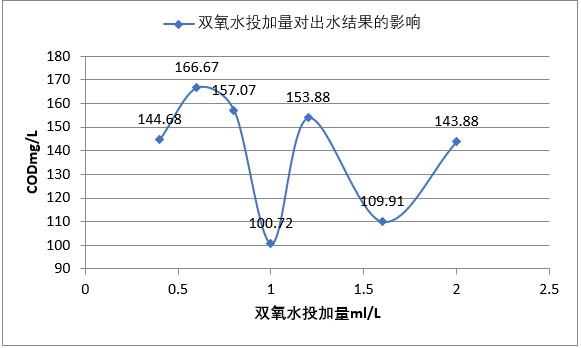
\includegraphics[width=150mm]{Img/fig2.jpg}\par}
{\hspace{40mm} 图2 硫化氢的进、出气浓度及去除率}\par
\vspace{10mm}
通过实验得出:在氨氮及硫化氢浓度在100ppmv以下,用生物滴滤池处理城市污水处理厂臭气运行效果良好。\par
 \\[120mm]
    \hline 
    \setlength{\parindent}{2em}
    {\bfseries下一步研究计划和任务:} \par
    试验的结论已基本呈现,Fenton技术属\showproject中的可行技术。课题正按照计划开展,进度无延误,可进行下一步的试验研究,后续的试验工作也将按原计划及思路继续开展。具体研究计划和任务如下:\par
现在至2018年6月,设计以Fenton工艺为基础的高级催化氧化一体化设备\par
2018年6月至2018年10月,设备交付加工并运输至\showprojectlocation现场\par
2018年10月至2018年11月,在\showprojectlocation现场进行调试与数据收集分析\par
2018年11月-2018年12月,验证试验总结、项目收尾并撰写结题报告\par \\[120mm]
    \hline 
    \setlength{\parindent}{2em}
    {\bfseries存在的问题、建议及其他需要说明的情况:} \par
    适合作为生物除臭工程验证的项目尚为找到。 \\[100mm]
\end{longtable}

\clearpage
\begin{mdframed}[subtitlebelowline=true,subtitleaboveline=true,subtitleaboveskip=-2mm,subtitlebelowskip=5mm,subtitleinneraboveskip=1mm,subtitleinnerbelowskip=1mm]
    \mdfsubtitle{\subsection*{总工程师意见}}
    课题研究顺利,取得成果较好,按照计划继续推进。\par
    \vspace*{200mm} 
    \noindent\hspace{100mm}总工程师:\par
    \noindent\hspace{100mm}20\qquad年\quad月\quad日
\end{mdframed}% main content
%-
%-> Backmatter: bibliography, glossary, index
%-


\end{document}